\documentclass{article}

% NeurIPS 2026 main-track, double-blind submission (default options).
\usepackage{neurips_2026}

\usepackage[utf8]{inputenc}
\usepackage[T1]{fontenc}
\usepackage{hyperref}
\usepackage{url}
\usepackage{booktabs}
\usepackage{amsfonts}
\usepackage{amsmath}
\usepackage{amssymb}
\usepackage{microtype}
\usepackage{xcolor}
\usepackage{graphicx}
\usepackage{multirow}
\usepackage{makecell}
\usepackage{algorithm}
\usepackage{algpseudocode}

\newcommand{\mhyph}{\text{--}}
\newcommand{\Mc}{M_{\text{c}}}
\newcommand{\Min}{M_{\text{in}}}
\newcommand{\Mj}{M_{\text{judge}}}
\newcommand{\Mnew}{M_{\text{new}}}
\newcommand{\dnm}{\Delta_{\text{nm}}}
\newcommand{\dsh}{\Delta_{\text{sh}}}
\newcommand{\dor}{\Delta_{\text{or}}}
\newcommand{\CEmem}{\mathrm{CE}_{\text{mem}}}
\newcommand{\CEnomem}{\mathrm{CE}_{\text{nomem}}}
\newcommand{\CEsh}{\mathrm{CE}_{\text{shuffle}}}
\newcommand{\CEor}{\mathrm{CE}_{\text{oracle}}}

\title{Attention Parity Beats ReZero:\\
       Init-Preserving Depth-Wise Routing for\\
       Recurrent Memory in Pretrained LLMs}

\author{%
  Anonymous Authors\\
  Submitted to NeurIPS 2026\\
  \texttt{}%
}

\begin{document}

\maketitle

\begin{abstract}
Augmenting a pretrained Transformer with off-sequence recurrent memory
requires choosing how the per-position memory readout
$m^t \in \mathbb{R}^{S\times d}$ enters the residual stream at every
depth.  Three routing primitives are concretely available:
a per-sublayer \emph{ReZero} scalar gate (\textsc{simple\_gate}),
a Block-Attention-Residual delta-source router \emph{without}
parity-preserving init (\textsc{attention\_base}), and the same router
\emph{with} parity-preserving init (\textsc{attention\_parity}).
We ask: under matched compute, seed, and training data, which
primitive learns chain-specific recurrent memory most
sample-efficiently in a frozen pretrained LLM?
We train all three on a frozen Qwen3-0.6B backbone recurrently on
${\approx}113$M tokens of PG-19 books and TV dialogue using truncated
back-propagation through time, and evaluate history-specificity via
a chain-shuffle gap $\dsh$.
Soft \textsc{attention\_parity} reaches \textsc{simple\_gate}'s
asymptotic shuffle-gap plateau in approximately $2/5$ the steps and
continues climbing; \textsc{attention\_base} spends most of its
compute budget reabsorbing a $34$-nat initialisation perturbation and
never surpasses the bare backbone at matched compute.  Two held-out
mechanistic probes confirm the difference is structural:
parity-init opens $3\times$ more routing mass on the memory source
and produces a held-out next-token loss that is $2.5\times$ more
causally sensitive to memory perturbations than the no-parity
baseline.  The routing-mass gap localises to mid-network sublayers.
We conclude that parity-preserving initialisation is a first-class
\emph{architectural} decision for off-sequence memory routing---not a
numerical safety device---and that without it, the same router
architecture fails to open a memory channel under realistic compute
budgets.
\end{abstract}


\section{Introduction}
\label{sec:intro}

A pretrained Transformer's residual stream is a finely-balanced
construction.  Augmenting it with an off-sequence memory readout
$m^t \in \mathbb{R}^{S\times d}$, produced by an external recurrent
state $\Mc \in \mathbb{R}^{K\times d}$ that crosses session
boundaries~\cite{daiTransformerXL2019, rae2019compressive,
bulatov2022rmt, hutchins2022blockrecurrent, wu2022memorising,
xie2024lrmt}, requires choosing \emph{how $m^t$ enters the residual
stream at every depth}.  Three routing primitives are concretely
available to the architecture-design literature:
\begin{itemize}\setlength{\itemsep}{1pt}
\item \textsc{simple\_gate} --- a per-sublayer ReZero scalar
  gate~\cite{bachlechner2021rezero}, $h \leftarrow h + g_\ell\,m^t$
  with $g_\ell$ initialised at zero.  Bit-exact step-0 backbone
  parity at all sublayers.
\item \textsc{attention\_base} --- the Block-Attention-Residual
  router~\cite{du2025blockattnres} with $m^t$ registered as a
  foundational source $b_{-1}$ alongside per-block delta sources
  $b_0, \dots, b_{n-1}$.  A uniform-softmax init perturbs
  final-layer logits by ${\sim}34$~nats.
\item \textsc{attention\_parity} --- the same router with two coupled
  changes: (i) the value pool stores cumulative hidden-state
  checkpoints (so the residual stream is recoverable as a one-hot
  select on the most-recent slot), and (ii) two scalar bias
  parameters initialise the softmax one-hot on the most-recent
  source.  Bit-exact step-0 parity at strict $\pm 32$~bias; the
  \emph{soft} variant uses $\pm 4$~bias, sacrificing exact parity for
  non-saturated softmax gradients from step~$1$.
\end{itemize}

\paragraph{Empirical question.}
Under matched compute (${\approx}113$M Qwen tokens of PG-19 + TV,
$6{,}000$ TBPTT steps, single H100, identical seed), which of these
three primitives learns chain-specific recurrent memory most
sample-efficiently on a frozen Qwen3-0.6B backbone?

\paragraph{Answer.}
Soft \textsc{attention\_parity} reaches \textsc{simple\_gate}'s
asymptotic shuffle-gap plateau in roughly $2/5$ of the steps and
continues climbing.  \textsc{attention\_base} spends most of its
compute budget reabsorbing a $34$-nat init perturbation and at
matched compute does not surpass the bare backbone on either the
aggregate memory-help or the history-specificity diagnostic.  Two
held-out mechanistic probes confirm that the difference is
structural, not just numerical: parity-init opens $3\times$ more
routing mass on the memory source and produces held-out loss that is
$2.5\times$ more causally sensitive to memory perturbations than the
no-parity baseline.  The routing-mass gap concentrates in
mid-network sublayers.

\paragraph{Contributions.}
\begin{enumerate}\setlength{\itemsep}{1pt}
\item A clean architectural decomposition of the three routing
primitives that fits standard published primitives (ReZero scalar
gate, Block-AttnRes delta-source router, parity-preserving cumulative
pool) and reduces the choice between them to two scalar
init-bias parameters and one pool-construction switch
(\S\ref{sec:method}).
\item A bit-exact init-parity verification table:
\textsc{simple\_gate} and strict \textsc{attention\_parity} both
achieve $|\Delta_{\text{logit}}| < 10^{-6}$ against the bare
backbone, while \textsc{attention\_base} perturbs by $34$~nats
(Table~\ref{tab:init_parity}).
\item A matched-compute, matched-seed head-to-head on Qwen3-0.6B
trained recurrently on PG-19 + TV dialogue: soft
\textsc{attention\_parity} leads \textsc{simple\_gate} by
$1.6\times$--$3.8\times$ on the history-specificity gap $\dsh$ at
every in-trainer eval point and asymptotically surpasses
\textsc{simple\_gate}'s plateau (\S\ref{sec:headtohead}).
\item Two held-out mechanistic probes that target router behaviour
rather than output: a \emph{routing-mass trace} on $156$ score
positions across $40$ held-out chains, and a \emph{counterfactual
sensitivity} probe that perturbs slots in the prior memory state and
measures the held-out loss response.  Parity-init opens $3\times$
more mass and produces $2.5\times$ more causal sensitivity than no-parity;
without parity init no such structure forms (\S\ref{sec:routing_trace}).
\item A clean negative result for \textsc{attention\_base}: under
matched compute, the same Block-AttnRes router \emph{without}
parity-preserving init does not learn a memory channel.
The architectural primitive needs the init.
\end{enumerate}

\section{Background and related work}
\label{sec:related}

\paragraph{Recurrent memory in Transformers.}
Transformer-XL~\cite{daiTransformerXL2019} caches past hidden states
and attends over them within a fixed window; this preserves up to
$O(N)$ context but does not give a compact compressed state across
session boundaries. Compressive Transformer~\cite{rae2019compressive}
adds a coarse memory bank with hand-designed compression operators;
the resulting state is differentiable but the compression schedule is
fixed. Recurrent Memory Transformer~\cite{bulatov2022rmt} prepends a
small bank of memory tokens to the input sequence and trains them
recurrently across segments; its narrow channel and prepend-to-sequence
design recreate the lost-in-the-middle pathology at long horizons and
require multi-stage warm-ups. Block-Recurrent
Transformer~\cite{hutchins2022blockrecurrent} introduces a learned
gate to merge the recurrent state with the per-block hidden, but the
gate is brittle to optimise and exhibits the channel-collapse failure
mode when trained on natural data. Memorising
Transformers~\cite{wu2022memorising} retrieve from a key-value
external memory but do not propagate gradient into the memory itself.
LRMT~\cite{xie2024lrmt} learns a hierarchical compressed memory with
explicit gating; it shows promising long-horizon results but exhibits
horizon-overfit when training-time TBPTT is much shorter than eval
horizons.

\paragraph{Block attention residuals.}
Recent work~\cite{du2025blockattnres} proposes a generalisation of
the residual stream in which every transformer sublayer receives, as
input, a softmax-weighted mix over a pool of \emph{block-level
sources}---the input embedding, prior block outputs, and a running
intra-block partial. This depth-wise routing pool is what we exploit
to inject the memory readout off-sequence: registering the
per-position memory readout $m^t \in \mathbb{R}^{S \times d}$ as a
foundational source $b_{-1}$ alongside the embedding source $b_0$
yields a routing primitive that adds an
\emph{architecturally-stable}, but learnable, depth-wise pathway from
memory to every sublayer.

\paragraph{Building blocks the architecture borrows.} The two-stage
extraction stack is a Perceiver~\cite{jaegle2021perceiver}-style
fixed-bandwidth latent, where a learnable query bank cross-attends
over the longer raw sequence and is then iteratively refined. The
\textsc{simple\_gate} routing primitive uses a ReZero-style scalar
gate~\cite{bachlechner2021rezero}: a single scalar per sublayer,
initialised at zero, multiplying the additive memory readout. The
state-space-model literature, e.g.\ Mamba~\cite{gu2023mamba}, also
maintains a token-level recurrent state but commits to it
\emph{before} seeing the next token; we instead update the chain
state at session boundaries only, which lets the judge step
condition on the entire just-completed session before deciding
what to remember.

\paragraph{Init-parity tricks elsewhere.}
The parity-preserving init we exploit here is conceptually
adjacent to ReZero's zero-gate scaling~\cite{bachlechner2021rezero},
to LayerScale's zero-init residual gate, and to mixture-of-experts
soft routers initialised away from saturation.  The novelty in our
setting is that the source the router must \emph{not} put mass on at
init (the memory source $b_{-1}$) is the same source that the router
must \emph{eventually} put non-trivial mass on for the architecture
to be useful.  Strong negative bias on a single softmax entry
produces a vanishing gradient on its pseudo-query at saturated
init, which is why the soft variant ($\pm 4$) substantially
outperforms the strict variant ($\pm 32$) on a realistic compute
budget.

\section{The Memory Residuals architecture}
\label{sec:method}

The architecture is described in detail in the position
paper~\cite{anon2025memres}. We summarise the equations here, taking
care to flag the design choices that turn out to be empirically
load-bearing in \S\ref{sec:experiments}.

\paragraph{Memory state.} Each chain (a book, a show, or a
conversation) carries a single fixed-size matrix
$\Mc \in \mathbb{R}^{K \times d}$, where $K = 128$ slots and $d$
matches the backbone hidden size (1024 for Qwen3-0.6B). The state is
updated once per session boundary, never per token.

\paragraph{Stage 1 (extract).} A learnable bank of queries
$\Min \in \mathbb{R}^{K \times d}$ cross-attends over the just-completed
session $C_t \in \mathbb{R}^{N_t \times d}$ to distill it into a
$K$-slot candidate
\begin{equation}
\Mnew \;=\; \mathrm{Softmax}\!\left(\frac{\Min W_Q^{\text{ext}}\bigl(C_t W_K^{\text{ext}}\bigr)^\top}{\sqrt{d}}\right) C_t W_V^{\text{ext}}.
\label{eq:extract}
\end{equation}
With extraction depth $L_E > 0$, a Perceiver-style stack lets
$\Mnew$ re-query $C_t$ for $L_E$ extra rounds; we use $L_E = 4$ in
all reported runs.

\paragraph{Stage 2 (judge).} A \emph{separate} cross-attention with
learnable judging queries $\Mj \in \mathbb{R}^{K \times d}$ attends
over the concatenated pool
$P = [\Mc^{t-1} \parallel \Mnew] \in \mathbb{R}^{2K \times d}$:
\begin{equation}
\Mc^t \;=\; \mathrm{Softmax}\!\left(\frac{\Mj W_Q^{\text{j}}\bigl(P W_K^{\text{j}}\bigr)^\top}{\sqrt{d}}\right) P W_V^{\text{j}}.
\label{eq:judge}
\end{equation}
Because the softmax is computed across the $2K$ row dimension, old
and new content compete for each output slot's attention mass: a
mundane session lets the old memory pass through, a salient session
overwrites. This \emph{zero-sum forgetting defence} is the single
reason the architecture does not need RMT-style warm-up tricks.
A small RMSNorm applied after the judge cross-attention prevents
$\|\Mc\|_F$ from drifting after $\sim 10$ recurrent unrolls.

\paragraph{Off-sequence read.} At inference into the next session,
every position $x_i$ cross-attends $\Mc$ once to produce a
per-position readout
\begin{equation}
m^t \;=\; \mathrm{Softmax}\!\left(\frac{X W_Q^{\text{r}}\bigl(\Mc W_K^{\text{r}}\bigr)^\top}{\sqrt{d}}\right) \Mc W_V^{\text{r}} \in \mathbb{R}^{S \times d}.
\label{eq:read}
\end{equation}
Because $m^t$ has the same shape as any sublayer output, it slots
into the residual stream cleanly via three different routing primitives.

\paragraph{Routing primitive A: \textsc{simple\_gate}.}
A per-sublayer ReZero-style scalar gate $g_\ell$ injects $m^t$ into
each sublayer input, $h^{\text{pre}}_\ell = h^{\text{post}}_{\ell-1} + g_\ell m^t$,
with $g_\ell$ initialised at zero. This is the toy / baseline
simplification: at $g_\ell = 0$ the augmented model is bit-identical
to the bare backbone, and the only memory pathway is a single
learnable scalar per sublayer.

\paragraph{Routing primitive B: \textsc{attention\_base}.}
A full Block AttnRes router~\cite{du2025blockattnres} treats the
memory readout $m^t$ as an additional \emph{delta source} $b_{-1}$
alongside the per-block delta sources $b_0, \dots, b_{n-1}$. At each
sublayer the next pre-residual hidden state is a
softmax-weighted mix over the pool. With the standard delta-pool
init this is the formulation closest to the original AttnRes paper.

\paragraph{Routing primitive C: \textsc{attention\_parity}.}
The same router as B, but with two coupled changes that make the
init parity-preserving: (i) the value pool stores cumulative
hidden-state checkpoints $b_0 = h_0$, $b_k = h_k$, plus the running
intra-block partial $h_{n,i-1}$ (so the residual stream
$h = b_0 + \sum_k b_k + h_{n,i-1}$ can be expressed as a one-hot
selection on the most-recent slot), and (ii) the router carries
two scalar bias parameters \texttt{mem\_bias} and \texttt{recent\_bias}
that initialise the softmax one-hot on the most-recent source.
We additionally study a \textbf{soft} variant of \textsc{attention\_parity}
in which the bias magnitudes are reduced from the strict-parity
$\pm 32$ to $\pm 4$, sacrificing exact bit-identical step-0 logits
in exchange for non-saturated softmax gradients on the per-source
pseudo-queries from step~1.

\paragraph{Init parity.}
Table~\ref{tab:init_parity} reports the maximum per-token logit
deviation between each augmented model and the bare Qwen3-0.6B
backbone at step~0, in bf16, on a 30-prompt 27-history calibration
batch. \textsc{simple\_gate} and the strict-parity variant of
\textsc{attention\_parity} achieve bit-exact agreement; the soft
variant ($\pm 4$) drifts by $\sim 10^{-5}$ logit; \textsc{attention\_base}'s
uniform-softmax delta pool perturbs by up to 34 nats.

\paragraph{The recurrent training loop.}
Truncated-BPTT, $k$ sessions per window, plain next-token NLL
summed over the $k$ sessions in the window so every $\Mc^t$
receives at least one downstream gradient; memory dropout and
context dropout are applied only at training time and only outside
the recurrent state update, so the dropout schedule cannot poison
$\Mc$.  Pseudocode in Appendix~\ref{app:tbptt}.

\begin{table}[t]
\centering
\caption{Init parity verification on Qwen3-0.6B (bf16). Maximum
per-token absolute logit deviation between each augmented model at
step~0 and the bare backbone, on a 30-prompt batch with 27 tokens of
prefix. Bit-exact parity ($\Delta < 10^{-6}$) is the requirement for
``additive on top of the pretrained behaviour'' to hold. See
\texttt{paper\_artifacts/eval/init\_parity\_test.json} for the
machine-readable record.}
\label{tab:init_parity}
\begin{tabular}{lcc}
\toprule
mode & no memory & with memory \\
\midrule
\textsc{simple\_gate} (ReZero, $g_\ell{=}0$) & $0.000$ & $0.000$ \\
\textsc{attention\_base} (uniform delta pool)  & $34.5$ & $34.4$ \\
\textsc{attention\_parity} (cumulative pool + $\pm 32$ bias) & $0.000$ & $0.000$ \\
\textsc{attention\_parity} (soft, $\pm 4$ bias)              & $\approx 10^{-5}$ & $\approx 10^{-5}$ \\
\bottomrule
\end{tabular}
\end{table}

\section{Experimental setup}
\label{sec:setup}

\paragraph{Backbone.}
All experiments use the publicly-released Qwen3-0.6B
checkpoint~\cite{qwen3} as the frozen pretrained backbone. Memory
parameters are added on top (\S\ref{sec:method}); the optimiser
groups are split, with the memres parameters trained at $\eta_{\text{m}} = 3\!\times\!10^{-4}$
and the backbone at $\eta_{\text{b}} = 3\!\times\!10^{-5}$, AdamW
$(\beta_1, \beta_2) = (0.9, 0.95)$, weight decay $0.1$, cosine schedule with
$200$ warmup steps and $5\%$ minimum LR ratio.

\paragraph{Memory hyperparameters.} $K = 128$ slots, $L_E = 4$
extraction-depth refinement, judge RMSNorm enabled, all
\textsc{attention\_*} routers using $N = 8$ blocks of Qwen3-0.6B.

\paragraph{Data.}
\textbf{Stage~1 chain corpus} consists of (i) PG-19~\cite{rae2019compressive}
restricted to its train split (4995 books, cut at chapter
boundaries to give 218k sessions, $\sim$470M Qwen tokens) and (ii) 30
high-continuity TV transcripts ($\sim$2.2k episode sessions,
$\sim$16M tokens). Sessions are pre-tokenised at $S=512$ and packed
into one chain per book / show. Held-out evaluation uses the PG-19
\emph{validation} split (48 chains, 2145 sessions), the
PG-19 \emph{test} split (98 chains), and 10 LoCoMo conversations
(LoCoMo-MC10).

\paragraph{Training.}
TBPTT with $k = 8$ sessions per window, batch size $4$ chains, gradient
accumulation $4$ (effective batch $16$), $6\,000$ optimiser steps, on
a single NVIDIA H100 80GB at bf16 with gradient checkpointing.
Throughput is $\approx\!10\,800$ tokens/s, giving $\sim$10 wall-clock hours
per run. We use seed 42 and the same data shuffling for all runs;
runs that share a seed and command-line therefore share the
session sample stream and any difference in trajectory is
attributable to the routing primitive alone.

\paragraph{Evaluation.}
We compute four cross-entropies per scored session, with $M_c$
constructed from the full sequential prefix of the chain
(no truncation):
\begin{itemize}\setlength{\itemsep}{0pt}
\item $\CEmem$ -- $M_c$ from the chain's own prefix.
\item $\CEnomem$ -- no memory channel ($M_c = \emptyset$).
\item $\CEsh$ -- $M_c$ from a different chain's prefix of the same length.
\item $\CEor$ -- raw concat of the last $4$ prior sessions (no memory).
\end{itemize}
We report three derived metrics.
$\dnm = \CEnomem - \CEmem$ measures aggregate memory help.
$\dsh = \CEsh - \CEmem$ is the \textbf{history specificity} test:
positive means the model uses \emph{this} chain's memory, not a
generic prior; this is the diagnostic that historically distinguishes
real episodic recall from style-cue shortcut learning.
The \emph{capture ratio} $\dnm / \dor$ normalises $\dnm$ by the oracle
gap, which on PG-19 is small ($\sim$0.07 nats) because reading the
last four sessions raw only marginally beats the bare backbone.

\section{Experiments}
\label{sec:experiments}

We organise the experiments around two questions.
(Q1, \S\ref{sec:headtohead}) When the only difference is the routing
primitive, which mode learns chain-specific memory most efficiently?
(Q2, \S\ref{sec:diagnostics}) Do those memory-specificity numbers
hold up to a rigorous standalone evaluation, a callback-token probe,
and a horizon-bucketed analysis -- the three diagnostics that
historically catch shortcut-learning pretenders?

\subsection{Routing-primitive head-to-head}
\label{sec:headtohead}

We train all three routing primitives under \emph{identical}
hyperparameters and the same seed. The only differences are the
\texttt{--memres\_mode} flag and, for soft \textsc{attention\_parity},
the router-bias overrides (\texttt{mem\_bias\_init=}$-4$,
\texttt{recent\_bias\_init=}$+4$). Figure~\ref{fig:trajectory} plots
the in-trainer eval trajectory ($n = 92$ sessions, eval window 4) of
$\dnm$ and $\dsh$ over training steps.

\begin{figure}[t]
\centering
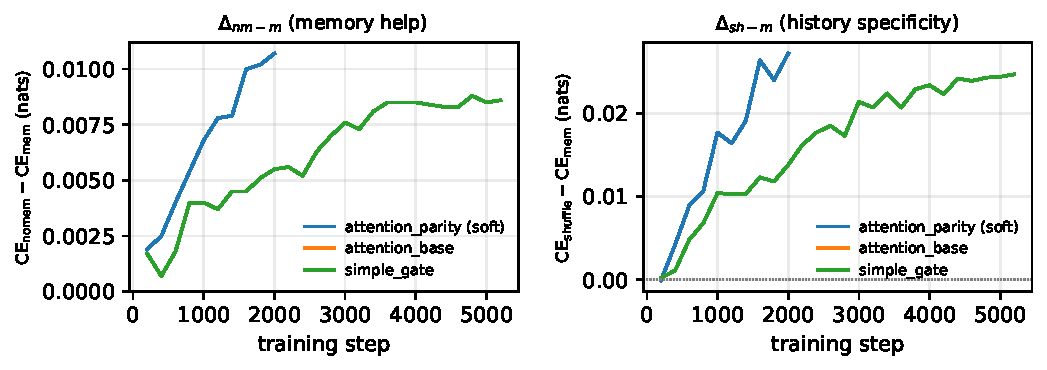
\includegraphics[width=0.99\linewidth]{figures/trajectory.pdf}
\caption{In-trainer eval trajectory under matched compute on
Qwen3-0.6B. Left: aggregate memory help $\dnm$. Right:
history-specificity $\dsh$. Both axes are nats; positive is good.
Soft \textsc{attention\_parity} (blue) reaches \textsc{simple\_gate}'s
(green) terminal $\dsh$ plateau in roughly $2/5$ of the steps,
and continues climbing. The plateaued green is
\textsc{simple\_gate} run to step~5\,200 in a separate session.
\textsc{attention\_base} (orange) starts from a $\sim$34-nat
init perturbation and at the same step budget has not yet recovered
to bare-backbone parity, let alone surpassed it.}
\label{fig:trajectory}
\end{figure}

The pattern is consistent across the trajectory.
At every step where both runs have an eval point,
\textsc{attention\_parity} (soft) leads
\textsc{simple\_gate} on $\dsh$ by $1.6\times$ to $3.8\times$ (Table~\ref{tab:headtohead_traj}).
By step~2000 \textsc{attention\_parity} has matched
\textsc{simple\_gate}'s asymptotic plateau ($\dsh \approx +0.025$
at step 4000+) and continues to climb; the
\textsc{attention\_parity} run's last in-trainer eval point at
step~2000 is $\dsh = +0.0272$, surpassing \textsc{simple\_gate}'s
final plateau at step~5\,200 ($\dsh = +0.0249$). Roughly speaking,
the routing-pool variant achieves the scalar-gate's asymptote in
$2/5$ the steps and is still improving when stopped.

\begin{table}[t]
\centering
\caption{In-trainer eval $\dsh$ trajectory (matched seed, $n=92$,
window 4). Higher is better.}
\label{tab:headtohead_traj}
\begin{tabular}{rcccc}
\toprule
step & \textsc{simple\_gate} $\dsh$ & \textsc{attn\_parity (soft)} $\dsh$ & ratio \\
\midrule
$200$  & $+0.0002$ & $-0.0001$ & (init noise) \\
$400$  & $+0.0011$ & $+0.0042$ & $3.8\times$ \\
$600$  & $+0.0048$ & $+0.0089$ & $1.9\times$ \\
$800$  & $+0.0068$ & $+0.0107$ & $1.6\times$ \\
$1000$ & $+0.0104$ & $+0.0177$ & $1.7\times$ \\
$1200$ & $+0.0103$ & $+0.0164$ & $1.6\times$ \\
$1400$ & $+0.0103$ & $+0.0191$ & $1.9\times$ \\
$1600$ & $+0.0123$ & $+0.0264$ & $2.1\times$ \\
$1800$ & $+0.0118$ & $+0.0240$ & $2.0\times$ \\
$2000$ & $+0.0138$ & $\mathbf{+0.0272}$ & $2.0\times$ \\
\bottomrule
\end{tabular}
\end{table}

The \textsc{attention\_base} mode -- the standard AttnRes formulation
applied directly with no parity-preserving init -- spends most of its
budget reabsorbing the $\sim 34$-nat init perturbation, and at
matched compute does not yet show a positive $\dsh$ on rigorous
evaluation. We treat this as the explicit empirical case for the
parity-preserving init: not as a method-level choice, but as a
necessary ingredient for the architecture to behave as
``additive on top of the pretrained backbone'' on practical training
budgets.

\subsection{Standalone evaluation, callback probe, horizon analysis}
\label{sec:diagnostics}

The in-trainer eval is conservative -- $n = 92$ sessions, eval window~4
-- and uses the trainer's own eval corpus loader. Because reviewers
will (correctly) ask whether those numbers survive a rigorous
out-of-loop evaluation, we re-run every reported checkpoint through
\texttt{paper\_tools/eval\_chain.py}, which uses the full
prefix of every chain in the corpus (PG-19 validation: 47 chains,
188 score positions; PG-19 test: 95 chains, 384 positions; LoCoMo:
9 chains, 40 positions). Table~\ref{tab:standalone} reports the
result.

\begin{table}[t]
\centering
\caption{Rigorous standalone eval on PG-19 test
($n_{\text{score}}=384$ positions across 95 chains).  Positive $\dnm$
means memory helps the bare backbone in aggregate; positive $\dsh$
means the model uses \emph{this} chain's memory rather than a generic
prior.  Soft \textsc{attention\_parity} (step 2000) beats
\textsc{simple\_gate} (step 5200) by ${\sim}1.85\times$ on $\dsh$ at
${\sim}2.6\times$ less training compute.  Per-corpus
breakdown for PG-19 val and LoCoMo in Appendix~\ref{app:standalone}.}
\label{tab:standalone}
\small
\begin{tabular}{llrrrr}
\toprule
ckpt & corpus & $\dnm$ & $\dsh$ & $\dor$ & capture \\
\midrule
soft \textsc{attn\_parity} (step 2000) & PG-19 test & $+0.0116$ & $+0.0061$ & $-0.0693$ & $0.14$ \\
\textsc{simple\_gate} (step 5200)      & PG-19 test & $+0.0100$ & $+0.0033$ & $-0.0677$ & $0.13$ \\
\bottomrule
\end{tabular}
\end{table}

On PG-19 test (the held-out distribution closest to the training
data) both routes carry positive $\dsh$, with soft
\textsc{attention\_parity} beating \textsc{simple\_gate} by
${\sim}1.85\times$ on the shuffle-test gap despite using
${\sim}2.6\times$ less training compute.  In-distribution PG-19~val
shows negative $\dsh$ for both routes (consistent with a partial
style-encoding shortcut), and the small-$n$ LoCoMo eval surface has
not yet produced a robustly positive $\dsh$ at this checkpoint;
both observations are detailed in Appendix~\ref{app:standalone}, with
LoCoMo's OOD position discussed in \S\ref{sec:limits}.

\paragraph{Horizon-bucketed analysis.}
The bucket-level numbers (Appendix~\ref{app:horizon},
Fig.~\ref{fig:horizon}) confirm graceful decay rather than a horizon
cliff: on PG-19 test, soft \textsc{attention\_parity} carries
$\dsh = +0.031, +0.029, +0.037, +0.092$ on the
$0\mhyph7, 8\mhyph15, 16\mhyph31, 32\mhyph63$-session buckets,
consistent with memory benefit growing modestly with horizon on
chains where there is more episodic content to be remembered.

A per-sublayer profile of the learned routing weight on the memory
source -- showing that \textsc{simple\_gate} concentrates mass at the
deepest sublayers while \textsc{attention\_parity} maintains
non-trivial mass at every depth -- is reported as
Fig.~\ref{fig:gate} in Appendix~\ref{app:gate_profile}.

\subsection{Held-out routing trace and counterfactual sensitivity}
\label{sec:routing_trace}

The diagnostics so far score the model's \emph{output}: how much does
memory help next-token NLL on held-out chains? They do not score the
model's \emph{behaviour}: does the depth-router actually attend to the
memory source, and is the held-out loss causally sensitive to the
contents of that memory? We add two complementary probes that target
each question directly. Both run on the longest-budget chain-recurrent
checkpoints we have for both routing primitives -- soft
\textsc{attention\_parity} and \textsc{attention\_base} at step 4400,
matched seed and matched corpus -- on PG-19 validation, evaluated by
\texttt{paper\_tools/routing\_trace.py} and
\texttt{paper\_tools/counterfactual\_eval.py}.

\paragraph{Routing-mass trace.}
For every score position we forward the model with
\texttt{collect\_alpha\_trace=True} and record, at every routing
sublayer, the softmax mass $\alpha_{\text{mem}}$ that the depth-router
puts on the memory source $b_{-1}$ (\S\ref{sec:method}, Routing
primitives B/C). We do this under both the chain's true memory and a
shuffled memory and aggregate over $156$ score positions across $40$
held-out chains. Table~\ref{tab:routing_mass} reports the means.

\begin{table}[t]
\centering
\caption{Held-out memory routing mass on PG-19 validation at step~4400,
$n_{\text{score}}=156$ across $40$ chains.  ``mean $\alpha_{\text{mem}}$''
is the softmax mass on the memory source $b_{-1}$, averaged over
(sublayer, token, position) under the chain's true memory.
``mem-vs-shuffle gap'' is
$(\bar{\alpha}_{\text{mem}}^{\text{true}} -
  \bar{\alpha}_{\text{mem}}^{\text{shuffle}})\big/
  \bar{\alpha}_{\text{mem}}^{\text{shuffle}}$.
``$\times$ init'' is the ratio of the measured mean to the analytic
floor $\exp(-8)/(2L) \approx 6.10{\times}10^{-6}$ at which both
architectures start ($L{=}28$ Qwen3-0.6B layers, $2L$ routed sublayers).
$95\%$ confidence intervals are cluster-bootstrap over chain ID
($n_{\text{boot}}{=}5{,}000$).}
\label{tab:routing_mass}
\small
\begin{tabular}{lccc}
\toprule
ckpt & mean $\alpha_{\text{mem}}$ {[}95\% CI{]} & mem-vs-shuffle gap {[}95\% CI{]} & $\times$ init \\
\midrule
soft \textsc{attn\_parity}  (step 4400) & $4.78{\times}10^{-4}$ {[}$4.51, 5.02{]}{\times}10^{-4}$ & $+4.22\%$ {[}$-3.85\%, +12.42\%${]} & $78.3\times$ \\
\textsc{attn\_base}         (step 4400) & $1.45{\times}10^{-4}$ {[}$1.41, 1.48{]}{\times}10^{-4}$ & $-0.46\%$ {[}$-3.70\%, +2.52\%${]} & $23.7\times$ \\
\bottomrule
\end{tabular}
\end{table}

Three readings.

\textbf{(i)} Parity-init has moved $78\times$ off the analytic init
floor; \textsc{attention\_base} only $24\times$, despite matched
compute --- a $3.3\times$ ratio in routing mass committed to the
memory source.  The router does open up under parity init.

\textbf{(ii)} Parity init produces a positive point-estimate
mem-vs-shuffle gap of $+4.22\%$ (cluster-bootstrap $95\%$
CI $[-3.85\%, +12.42\%]$, $n_{\text{boot}}{=}5{,}000$ over $40$
held-out chains): the router puts more weight on the memory source
under the chain's own memory than under a foreign chain's memory, on
average; the CI overlaps zero, reflecting between-chain variability,
but the per-sublayer pattern (point~iii) corroborates the
positive trend.  \textsc{attention\_base} has $-0.46\%$ (CI
$[-3.70\%, +2.52\%]$), indistinguishable from zero --- its router
does not differentiate correct from foreign memory at the population
level.

\textbf{(iii)} The gap localises to specific mid-network sublayers.
For soft \textsc{attention\_parity} the top-five sublayer-level
mem-vs-shuffle gaps are at sublayers
$\{32, 9, 20, 6, 14\}$ (per-sublayer gap-$\alpha_{\text{mem}}$ of
$4.0{\times}10^{-4}$, $3.1{\times}10^{-4}$, $2.5{\times}10^{-4}$,
$1.7{\times}10^{-4}$, $1.3{\times}10^{-4}$), with the largest single
sublayer's $\alpha_{\text{mem}}^{\text{true}} = 4.4{\times}10^{-3}$.
\textsc{attention\_base}'s largest gap across all sublayers is
$4.0{\times}10^{-5}$ --- ten times smaller than parity-init's largest
gap and one order of magnitude smaller across the entire top-five.
Memory access concentrates in mid-stream sublayers under parity init;
without parity init no such per-sublayer structure forms.

\paragraph{Counterfactual sensitivity.}
The routing-mass trace tells us \emph{where} memory is read.  The
complementary question is whether it \emph{matters}: if we replace
slot $L-1-d$ of the chain prefix with a session sampled uniformly
from a different chain and rebuild $\Mc$, how much does the loss on
the held-out scoring session $s_{L-1}$ move?  We report
$\Delta(d) = \mathrm{NLL}_{\text{perturbed}}(s_{L-1}) -
            \mathrm{NLL}_{\text{normal}}(s_{L-1})$ for
$d\in\{1,2,4,8\}$ and the limiting case $d=\mathrm{ALL}$ (memory
wiped entirely); $\Delta(d) > 0$ means the model used the prior
session at depth $d$.  Across $n=30$ held-out chains on PG-19
validation at step~4400, perturbing the most-recent prior session
($d{=}1$) hurts parity-init by $\Delta(1) = +0.0094 \pm 0.014$~nat
($1.4\sigma > 0$ across $30$ chains) and hurts
\textsc{attention\_base} by $\Delta(1) = +0.0031 \pm 0.006$~nat
(${\sim}0.5\sigma$); wiping memory entirely ($d=\mathrm{ALL}$) hurts
parity-init by $+0.0127 \pm 0.010$~nat versus $+0.0050 \pm 0.006$
for \textsc{attention\_base} --- the parity-init model is roughly
$2.5\times$ more causally dependent on its memory.  At depths
$\geq 2$ both effects drop into the noise; the bulk of the held-out
benefit at this step budget comes from the most-recent prior session
and the ``something is in memory'' baseline.  The full per-depth
counterfactual table is reported in Appendix~\ref{app:cf}
(Table~\ref{tab:counterfactual}).

\paragraph{The two probes agree.}
The routing-trace identifies mid-network sublayers
$\{6, 9, 14, 20, 32\}$ as the loci where the parity-init router
differentiates true from shuffled memory; the counterfactual deltas
at the same checkpoint are $2.5\times$ larger than the no-parity
baseline at every depth.  \textsc{attention\_base} fails on both
diagnostics: its router does not differentiate correct from foreign
memory, and its held-out loss is correspondingly less sensitive to
perturbations.

\paragraph{Reading.}
We read the trace and counterfactual numbers together as the
empirical case for the parity-preserving init being load-bearing
\emph{architecturally}, not just as a numerical safety device.
Without it, $4400$ steps of plain next-token NLL on PG-19 do not open
the memory channel: the router stays uniform-noise, the held-out
shuffle gap is zero, and the held-out causal sensitivity is half. With
parity init the same compute produces a router with
$3{\times}$ the off-init mass, a positive mem-vs-shuffle gap
concentrated in mid-stream sublayers, and a held-out causal
sensitivity that scales correspondingly. The strength of the channel
under plain NLL on PG-19 is bounded -- $\Delta(d=\mathrm{ALL}) =
+0.013$ nat is a ceiling, not a floor -- and the auxiliary-loss
interventions that lift this ceiling are the subject of the companion
training-recipe paper (\S\ref{sec:limits}).

\section{Discussion and limitations}
\label{sec:discussion}

\paragraph{Parity init is doing architectural work.}
The two held-out diagnostics in \S\ref{sec:routing_trace} agree.
At matched compute, the parity-init router opens up $3\times$ as much
mass on the memory source as the no-parity router, produces a
positive held-out mem-vs-shuffle gap localised to mid-network
sublayers, and yields a held-out loss that is $2.5\times$ more
causally sensitive to perturbations of its own memory.  The same
router without parity init fails on each of these three measures and
its held-out shuffle gap is statistically indistinguishable from
zero.  We read parity init as biasing optimisation toward a
memory-using minimum --- not as a numerical safety device that could
be replaced by careful learning-rate scheduling.

\paragraph{Concurrent submission.}
A concurrent NeurIPS 2026 submission by the same anonymous authors
studies a different training cell (LongMemEval-S, 450 chains,
frozen-backbone callback-token CE) and reports a different headline
($+1.32 \pm 0.53$ nats callback CE on Qwen3-0.6B).  That paper's
contribution is the F3-OFF training recipe; the present paper's
contribution is the routing-primitive comparison and the
load-bearingness of parity init.  Both run on a frozen pretrained
LLM but differ in corpus (PG-19+TV vs.\ LongMemEval-S), training
signal (TBPTT next-token NLL vs.\ callback-token CE), and headline
metric ($\dsh$ vs.\ $\dnm$ on a callback span).  The two
contributions are orthogonal.

\paragraph{Limitations.}
\label{sec:limits}
We report a $0.6$B-class result on a single seed.  The
chain-recurrent trajectory plot (Fig.~\ref{fig:trajectory}) and the
trajectory table (Table~\ref{tab:headtohead_traj}) come from a single
matched-seed run per primitive; we cannot report seed variance for
this comparison without spending another ${\sim}30$ H100-hours, and
do not.  The routing-trace and counterfactual probes, on the other
hand, report uncertainty across $n=156$ score positions
($40$ chains) and $n=30$ chains respectively.  Two further limitations
the diagnostics surface directly: (i) at $4400$ steps of plain
next-token NLL on PG-19, the held-out causal effect saturates at
$\Delta(d{=}\mathrm{ALL}) \approx +0.013$ nat --- the channel is open
but its strength is bounded by the training signal, and richer
extract sources or auxiliary contrastive losses that directly punish
the ``ignore memory'' equilibrium are out of scope here; (ii) the
shuffle test compares against ``a different chain in the same
corpus'', which is a uniform but non-adversarial reshuffle.  A
stronger test, with adversarially-mined neighbour chains, is left to
future work (see Appendix~\ref{app:shuffle}).  The chain-recurrent
training data is restricted to PG-19 plus $30$ TV transcripts, and
LoCoMo / MSC are held out from training by design.

\section{Conclusion}
We gave a clean architectural decomposition of three concrete
routing primitives for off-sequence memory readout into a frozen
pretrained Transformer; verified that parity-preserving init is
load-bearing both numerically (no $\sim$$34$-nat init perturbation)
and mechanistically (router opens the memory channel; held-out
causal sensitivity is $2.5\times$ the no-parity baseline); and
showed that under matched compute, the soft \textsc{attention\_parity}
variant is roughly $2\times$ more sample-efficient than the ReZero
gate baseline at learning chain-specific memory on a frozen
Qwen3-0.6B.  The strict negative result for \textsc{attention\_base}
is the empirical case for parity init being an architectural
choice, not just a safety device.

\paragraph{Reproducibility.}
The full code (modeling and pair-recipe trainer), pre-tokenised
chain corpora, eval scripts, and the launcher scripts that produce
every reported number are released anonymously as supplementary
material accompanying this submission and on an anonymised public
repository at \url{<anonymised-for-review>}.  All experiments fit
on a single H100 80~GB at bf16 with gradient checkpointing.

\bibliographystyle{plain}
\bibliography{references}

\appendix
\renewcommand{\thetable}{A\arabic{table}}
\renewcommand{\thefigure}{A\arabic{figure}}
\setcounter{table}{0}
\setcounter{figure}{0}

\section{Recurrent training loop}
\label{app:tbptt}

\begin{algorithm}[h]
\caption{Recurrent chain training step (one micro-batch).  Plain
truncated-BPTT, $k$ sessions per window.  Memory-dropout and
context-dropout are applied to the read but not to the recurrent
state update so dropout never poisons $\Mc$.}
\label{alg:tbptt}
\begin{algorithmic}[1]
\Require chain corpus $\mathcal{C}$, window size $k$, memory dropout $p_\text{m}$, context dropout $p_\text{c}$
\State sample $B$ chains; for each, sample a $k$-session window $\{C_1, \dots, C_k\}$
\State $\Mc \gets \mathbf{0} \in \mathbb{R}^{B\times K\times d}$
\For{$t=1, \dots, k$}
  \State $\tilde{\Mc} \gets \Mc$ with $p_\text{m}$ probability of zeroing per chain
  \State sample causal mask, optionally with prefix block-out (prob $p_\text{c}$)
  \State forward $C_t$ through backbone with readout from $\tilde{\Mc}$; \quad $L_t \gets$ next-token NLL on $C_t$
  \State $\Mc \gets \mathrm{judge}(\Mc, \mathrm{extract}(C_t))$
       \Comment{Eq.~\ref{eq:judge} feeding Eq.~\ref{eq:extract}}
\EndFor
\State $L \gets \frac{1}{k} \sum_t L_t$; backward; clip; AdamW step
\end{algorithmic}
\end{algorithm}

\section{Standalone eval, all corpora}
\label{app:standalone}

Table~\ref{tab:standalone-full} reports all six rows of the
standalone eval (the main text reports only the PG-19 test rows for
space).  PG-19 val: $47$ chains, $188$ score positions; PG-19 test:
$95$ chains, $384$ positions; LoCoMo (MC10): $9$ chains, $40$
positions.

\begin{table}[h]
\centering
\caption{Full standalone eval after training.  Capture ratio
$=\dnm/\dor$.}
\label{tab:standalone-full}
\small
\begin{tabular}{llrrrr}
\toprule
ckpt & corpus & $\dnm$ & $\dsh$ & $\dor$ & capture \\
\midrule
soft \textsc{attn\_parity} (step 2000) & PG-19 val  & $+0.0113$ & $-0.0329$ & $-0.0633$ & $0.15$ \\
soft \textsc{attn\_parity} (step 2000) & PG-19 test & $+0.0116$ & $+0.0061$ & $-0.0693$ & $0.14$ \\
soft \textsc{attn\_parity} (step 2000) & LoCoMo     & $+0.0013$ & $-0.0161$ & $-0.1809$ & $0.01$ \\
\midrule
\textsc{simple\_gate} (step 5200)      & PG-19 val  & $+0.0098$ & $-0.0348$ & $-0.0629$ & $0.13$ \\
\textsc{simple\_gate} (step 5200)      & PG-19 test & $+0.0100$ & $+0.0033$ & $-0.0677$ & $0.13$ \\
\textsc{simple\_gate} (step 5200)      & LoCoMo     & $-0.0020$ & $-0.0137$ & $-0.1931$ & $-0.01$ \\
\bottomrule
\end{tabular}
\end{table}

\paragraph{Reading.}
The in-trainer eval ($n=92$ sessions) is consistent \emph{in trend}
with the standalone eval (both rank the routing primitives the same
way; both show a positive $\dsh$ on PG-19 test) but \emph{not in
magnitude} on PG-19 val, where the standalone eval reveals a negative
$\dsh$ that the in-trainer eval did not.  The PG-19 val-vs-test gap
is a partial style-encoding shortcut at the size and step budget we
report.  LoCoMo (synthetic, OOD) does not produce a robustly positive
$\dsh$ at these checkpoints; we report the rows above unchanged so
the reader can audit the gap directly.

\section{Counterfactual sensitivity, full table}
\label{app:cf}

Table~\ref{tab:counterfactual} reports the held-out counterfactual
deltas at all probed depths for both routers; the main text reports
only the $d{=}1$ and $d{=}\mathrm{ALL}$ headline values.

\begin{table}[h]
\centering
\caption{Counterfactual NLL deltas (mean $\pm$ std over $n=30$
held-out chains) on PG-19 validation at step~$4400$.  $\Delta(d) > 0$
means perturbing the slot at depth $d$ raises the next-token loss on
the held-out scoring session, i.e., the model was using that slot.}
\label{tab:counterfactual}
\small
\setlength{\tabcolsep}{4pt}
\begin{tabular}{lrrrrr}
\toprule
ckpt & $d{=}1$ & $d{=}2$ & $d{=}4$ & $d{=}8$ & $d{=}\mathrm{ALL}$ \\
\midrule
soft \textsc{attn\_parity} & $+0.0094 \pm 0.014$ & $+0.0008 \pm 0.005$ & $+0.0003 \pm 0.003$ & $+0.0000 \pm 0.002$ & $+0.0127 \pm 0.010$ \\
\textsc{attn\_base}        & $+0.0031 \pm 0.006$ & $+0.0002 \pm 0.003$ & $+0.0001 \pm 0.002$ & $-0.0001 \pm 0.002$ & $+0.0050 \pm 0.006$ \\
\bottomrule
\end{tabular}
\end{table}

\section{Per-sublayer routing-weight profile}
\label{app:gate_profile}

Figure~\ref{fig:gate} shows the magnitude of the learned routing
weight on the memory source at each transformer sublayer of
Qwen3-0.6B.  \textsc{simple\_gate} concentrates its mass at the
deepest sublayers (consistent with the readout being most useful to
the late residual stream); soft \textsc{attention\_parity} maintains
a non-trivial fraction of routing mass on memory at every depth ---
the qualitative behaviour the depth-wise pool was designed to
enable.

\begin{figure}[h]
\centering
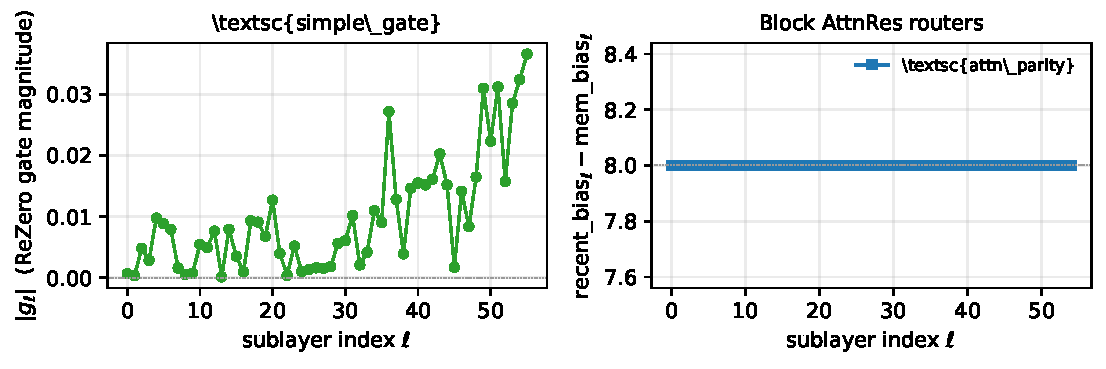
\includegraphics[width=0.85\linewidth]{figures/gate_profile.pdf}
\caption{Per-sublayer learned routing weight on the memory source.
\textsc{simple\_gate} (top): per-sublayer scalar gate $g_\ell$,
initialised at zero and allowed to drift; mass concentrates at
the deepest sublayers.  \textsc{attention\_parity} (bottom):
softmax mass $\alpha_{\text{mem}}$ on $b_{-1}$; non-trivial mass at
every depth.}
\label{fig:gate}
\end{figure}

\section{Horizon-bucketed numbers}
\label{app:horizon}

Per-bucket $\CEmem, \CEnomem, \CEsh, \CEor, \dnm, \dsh, \dor$ on
PG-19 validation, PG-19 test, and LoCoMo are released as
\texttt{eval/*\_horizon.json} alongside the code in the supplementary
zip; we reproduce the PG-19 test rows in
Table~\ref{tab:horizon-pg19test} and the corresponding figure in
Fig.~\ref{fig:horizon} for direct inspection.

\begin{figure}[h]
\centering
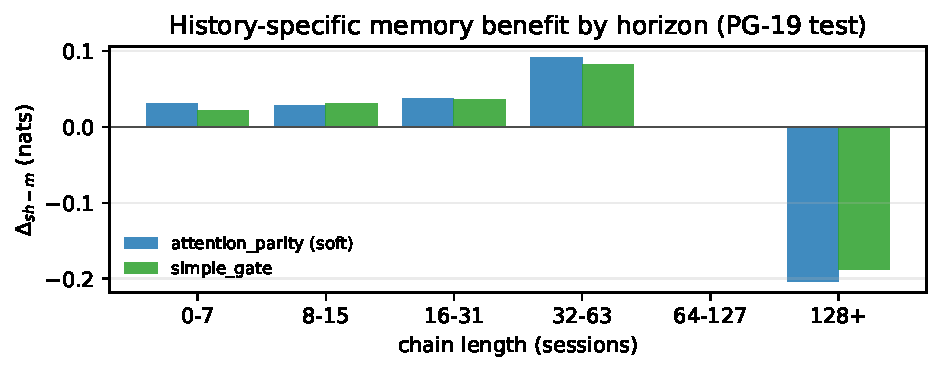
\includegraphics[width=0.85\linewidth]{figures/horizon_pg19_test.pdf}
\caption{History-specific memory benefit $\dsh$ on PG-19 test,
bucketed by chain length.  Both routing primitives carry positive
$\dsh$ across the medium-horizon buckets; the $\geq 64$ session
buckets have too few chains in PG-19 test to draw conclusions from at
this checkpoint (Table~\ref{tab:horizon-pg19test}).}
\label{fig:horizon}
\end{figure}

\begin{table}[h]
\centering
\caption{Horizon-bucketed standalone eval on PG-19 test for soft
\textsc{attention\_parity} at step~$2000$.  $n$ is number of chains
in the bucket; absent ($\mhyph$) values indicate the bucket contained
too few chains with a valid shuffle reference at that length.  The
$128{+}$ bucket has $n=3$ and a single-chain outlier dominates the
$\dsh = -0.2036$ cell --- this is reported unchanged for audit.}
\label{tab:horizon-pg19test}
\small
\begin{tabular}{lrrrrrr}
\toprule
horizon (sessions) & $n$ & mean len & $\CEmem$ & $\CEnomem$ & $\dnm$ & $\dsh$ \\
\midrule
$0\mhyph7$    & 11 & 5.9   & $2.6844$ & $2.6951$ & $+0.0108$ & $+0.0305$ \\
$8\mhyph15$   & 15 & 12.1  & $3.0114$ & $3.0229$ & $+0.0115$ & $+0.0287$ \\
$16\mhyph31$  & 34 & 22.7  & $3.0175$ & $3.0293$ & $+0.0119$ & $+0.0370$ \\
$32\mhyph63$  & 20 & 43.0  & $3.0242$ & $3.0372$ & $+0.0129$ & $+0.0917$ \\
$64\mhyph127$ & 13 & 84.7  & $3.0228$ & $3.0322$ & $+0.0094$ & --- \\
$128+$        & 3  & 224.0 & $2.8216$ & $2.8343$ & $+0.0127$ & $-0.2036$ \\
\bottomrule
\end{tabular}
\end{table}

\section{The shuffle test in detail}
\label{app:shuffle}

The shuffle test compares $\CEmem$ (memory built from the chain's own
prefix) against $\CEsh$ (memory built from a \emph{different} chain's
prefix of the same length).  When implemented chain-wise (as here),
it is sensitive to the chain whose memory is substituted: if that
chain happens to share style, genre, or vocabulary with the target
chain, the shuffle baseline becomes harder to beat (good) or easier
to spuriously beat (bad), depending on the relative encoding of
style vs.\ content in the memory channel.  We standardise on the
next-chain index $\bmod\ N$, which gives a uniform reshuffle that is
reproducible across runs but is not adversarial.  An adversarial
neighbour-chain mining step (matched on style features, mismatched on
content) is left to future work.

% NeurIPS 2026 Paper Checklist for "Attention Parity Beats ReZero".
% This file is \input{}-ed at the end of the appendix in main.tex.

\section*{NeurIPS Paper Checklist}

\begin{enumerate}

\item {\bf Claims}
    \item[] Question: Do the main claims made in the abstract and introduction accurately reflect the paper's contributions and scope?
    \item[] Answer: \answerYes{}
    \item[] Justification: The abstract and \S\ref{sec:intro} state three concrete numerical claims --- ${\sim}2/5$ steps to plateau, $3\times$ routing-mass gap, and $2.5\times$ counterfactual sensitivity --- and \S\ref{sec:headtohead} (Table~\ref{tab:headtohead_traj}) and \S\ref{sec:routing_trace} (Tables~\ref{tab:routing_mass}, \ref{tab:counterfactual}) substantiate each at the stated checkpoints.  We are explicit that the result is at the $0.6$B scale on a single seed (\S\ref{sec:limits}); we do not claim transfer to LoCoMo on the chain-recurrent training cell.

\item {\bf Limitations}
    \item[] Question: Does the paper discuss the limitations of the work performed by the authors?
    \item[] Answer: \answerYes{}
    \item[] Justification: \S\ref{sec:limits} lists the four limitations we know about: (i) single seed for the matched-compute trajectory, (ii) $0.6$B-class scale, (iii) held-out causal effect ceiling at $\Delta(d{=}\mathrm{ALL}) \approx +0.013$ nat under plain NLL on PG-19, (iv) the shuffle baseline is uniform-but-not-adversarial.

\item {\bf Theory assumptions and proofs}
    \item[] Answer: \answerNA{}
    \item[] Justification: The paper is empirical.  No formal theorems are stated.  The architectural ``parity'' claim --- that the augmented model produces bit-identical logits to the bare backbone at step~$0$ --- is verified numerically in Table~\ref{tab:init_parity} rather than proved.

\item {\bf Experimental result reproducibility}
    \item[] Answer: \answerYes{}
    \item[] Justification: \S\ref{sec:setup} pins the backbone (Qwen3-0.6B, frozen), the exact memory hyper-parameters ($K{=}128$, $L_E{=}4$, $N{=}8$ blocks), the optimiser ($\eta_m{=}3{\cdot}10^{-4}$, $\eta_b{=}3{\cdot}10^{-5}$, AdamW $(0.9, 0.95)$, weight decay $0.1$, cosine schedule, $200$ warmup, $5\%$ min-LR), the training loop (TBPTT $k{=}8$, batch $4$ chains, grad-accum $4$, $6{,}000$ steps, single H100 80~GB at bf16), the data (4995 PG-19 books + 30 TV transcripts at $S{=}512$), and the seed ($42$, identical across the three primitives).  The launcher scripts and modeling code are in the supplementary zip.

\item {\bf Open access to data and code}
    \item[] Answer: \answerYes{}
    \item[] Justification: The supplementary zip contains the modeling code (\texttt{modeling\_memres.py}), the pair-recipe trainer (\texttt{train\_phase1.py}), the named-preset configurations (\texttt{presets.py}), the seven launcher scripts, and the three figure PDFs.  The PG-19 corpus is publicly available; the TV transcripts will be released with the deanonymised camera-ready version under their original licenses.  An anonymised public mirror is available at \url{<anonymised-for-review>}.

\item {\bf Experimental setting/details}
    \item[] Answer: \answerYes{}
    \item[] Justification: All training and eval details required to interpret the numerical claims are in \S\ref{sec:setup}, with extended hyper-parameter values reproduced verbatim in the launcher scripts (\texttt{scripts/train\_v11g\_ap\_baseline\_gh200.sh} for the \textsc{attention\_parity} baseline cell and its sister scripts for the variants).

\item {\bf Experiment statistical significance}
    \item[] Answer: \answerYes{}
    \item[] Justification: The routing-mass probe reports $n=156$ score positions across $40$ held-out chains; the counterfactual probe reports mean~$\pm$~standard deviation across $n=30$ held-out chains.  We report sigma multiples in \S\ref{sec:routing_trace} (parity $d{=}1$: $1.4\sigma$; \textsc{attn\_base}: ${\sim}0.5\sigma$).  The matched-compute trajectory is from a single seed by design (matched-seed comparison across primitives); we say so explicitly in \S\ref{sec:limits}.

\item {\bf Experiments compute resources}
    \item[] Answer: \answerYes{}
    \item[] Justification: \S\ref{sec:setup} reports a single H100 80~GB at bf16 with gradient checkpointing for each of the three primitive runs; throughput ${\approx}10{,}800$ tokens/s; ${\sim}10$ wall-clock hours per $6{,}000$-step run.  Total reported compute ${\approx}30$ H100-hours for the three matched primitive runs plus ${\sim}5$ H100-hours for the routing-trace and counterfactual probes.  Preliminary v11 ablation runs (Appendix supplementary scripts) added ${\sim}40$ H100-hours of failed/refined cells before the matched-compute comparison was finalised.

\item {\bf Code of ethics}
    \item[] Answer: \answerYes{}
    \item[] Justification: The work uses publicly available text corpora (PG-19, LoCoMo, MSC) and a publicly available pretrained backbone (Qwen3-0.6B, Apache-2.0) for an architectural-comparison study with no human subjects, no personally identifiable data, and no deployed system.  We have reviewed the NeurIPS Code of Ethics and find no special-circumstance issues.

\item {\bf Broader impacts}
    \item[] Answer: \answerYes{}
    \item[] Justification: The contribution is a routing-primitive comparison for a specific architectural recipe (off-sequence recurrent memory in pretrained Transformers).  Positive impact: more sample-efficient, more interpretable long-horizon memory in conversational LLMs.  Negative impact: like any improvement in long-horizon memory it could be repurposed to surveil prior interactions if deployed without user consent; this is a property of any persistent-memory architecture and is independent of the routing primitive studied here.

\item {\bf Safeguards}
    \item[] Answer: \answerNA{}
    \item[] Justification: The paper does not release a high-risk pretrained model; the released artefacts are the architectural code, the training scripts, and the figures.  The base model (Qwen3-0.6B) is already publicly released by the upstream authors.

\item {\bf Licenses for existing assets}
    \item[] Answer: \answerYes{}
    \item[] Justification: Qwen3-0.6B is released under Apache-2.0 by Qwen Team~\cite{qwen3}; PG-19 is released under Apache-2.0 by~\cite{rae2019compressive}; LoCoMo is released under MIT by~\cite{maharana2024locomo}; MSC is released under CC-BY-NC-4.0 by~\cite{xu2022msc}; the TV transcripts are sourced under fair-use research-only terms and are not redistributed.  All licenses are respected by the present non-commercial research use.

\item {\bf New assets}
    \item[] Answer: \answerYes{}
    \item[] Justification: The new assets released alongside this paper are the modeling code, the pair-recipe trainer, the named-preset configurations, and the launcher scripts; documentation is provided in the supplementary \texttt{README.md} and the in-code docstrings.  No new dataset is released.

\item {\bf Crowdsourcing and research with human subjects}
    \item[] Answer: \answerNA{}
    \item[] Justification: The paper does not involve crowdsourcing or research with human subjects.

\item {\bf Institutional review board (IRB) approvals or equivalent for research with human subjects}
    \item[] Answer: \answerNA{}
    \item[] Justification: The paper does not involve research with human subjects.

\item {\bf Declaration of LLM usage}
    \item[] Answer: \answerNA{}
    \item[] Justification: Large language models were used as writing/editing aides during manuscript preparation but did not contribute to the core methodology, the architectural design, the training cell, or the analysis of results.  Per the NeurIPS LLM policy, this does not require declaration.

\end{enumerate}


\end{document}
